\chapter{Results}
\label{chap:Results}
%Include your results either in figure form or in a table. Remember to label your results.
%All tables and figures should have relevant captions and labels on the axes.


\subsection{ACE}

The magnetic field strength is shown in figure \figref{fig:ACE_MFI}. Here it's possible to see when an outburst from the sun is passing before it hits Earth. 

\begin{figure}[h!]
\centering
\begin{minipage}{0.49\textwidth}
\includegraphics[width=\textwidth]{Figures/ACE/AC_H0_MFI_19370_000.pdf}
\caption{Magnetometer showing field strength from ACE}
\label{fig:ACE_MFI}
\end{minipage}
\begin{minipage}{0.49\textwidth}
\includegraphics[width = \textwidth]{Figures/ACE/AC_H0_SWE_19370_001.pdf}
\caption{Bulk flow speed of the solar wind}
\label{fig:ACE_SWE}
\end{minipage}
\end{figure}

The most interesting part is the Bz component that is the field aligned component of the IMF. When the component is negative over a period of time then reconnection can take place.

It is negative over the period between 9.00 and 12.00, and also between 12.30 and 14.00. As can be seen in \figref{fig:ACE_MFI}.  

From \figref{fig:ACE_SWE} the velocity at which the solar wind travels towards Earth can be seen This velocity is about 340 $\frac{\textrm{km}}{\textrm{s}}$ for the first period between 9.00 and 12.00. For the second period between 12.30 and 14.00 the wind velocity is slightly lower at about 330 $\frac{\textrm{km}}{\textrm{s}}$. 




\subsection{Ground-Based Magnetometers}

The ground based magnetometers in \figref{fig:GBM} shows the magnetograms from the Svalbard area. In the magnetograms it's possible to see a decrease in the magnetic field strength starting at the station in Ny \AA lesund and the moving south ending at Bj\o rn \o ya. It starts at around 10.00 in Ny \AA lesund and goes down until 12.00, when it starts going back up before going down again between 14.00 and 15.30. 

On Hopen (HOP) it starts decreasing at around 12.00 and decreases until 13.00, when it stays quite stable during the rest of the period.

On Bj\o rn \o ya it starts decreasing around 12.00 and continues until 14.00 when it gains a bit strength before it decreases from 15.00 until 15.30. 

\begin{figure}[ht!]
\centering
\includegraphics[width=0.4\textwidth]{Figures/Magnetogram/Z_gram.jpg}
\caption{Magnetogram from Svalbard area}
\label{fig:GBM}
\end{figure}


\subsection{SuperDARN}

In \figref{fig:SD1415} the motion of plasma in the F-region is mapped at the time 14.15 UT. Here it's possible to see that there is a movement going eastward above Svalbard and across the polar cap from Russia to Canada. There is a twin cell pattern in the movement. 

\begin{figure}[ht!]
\centering
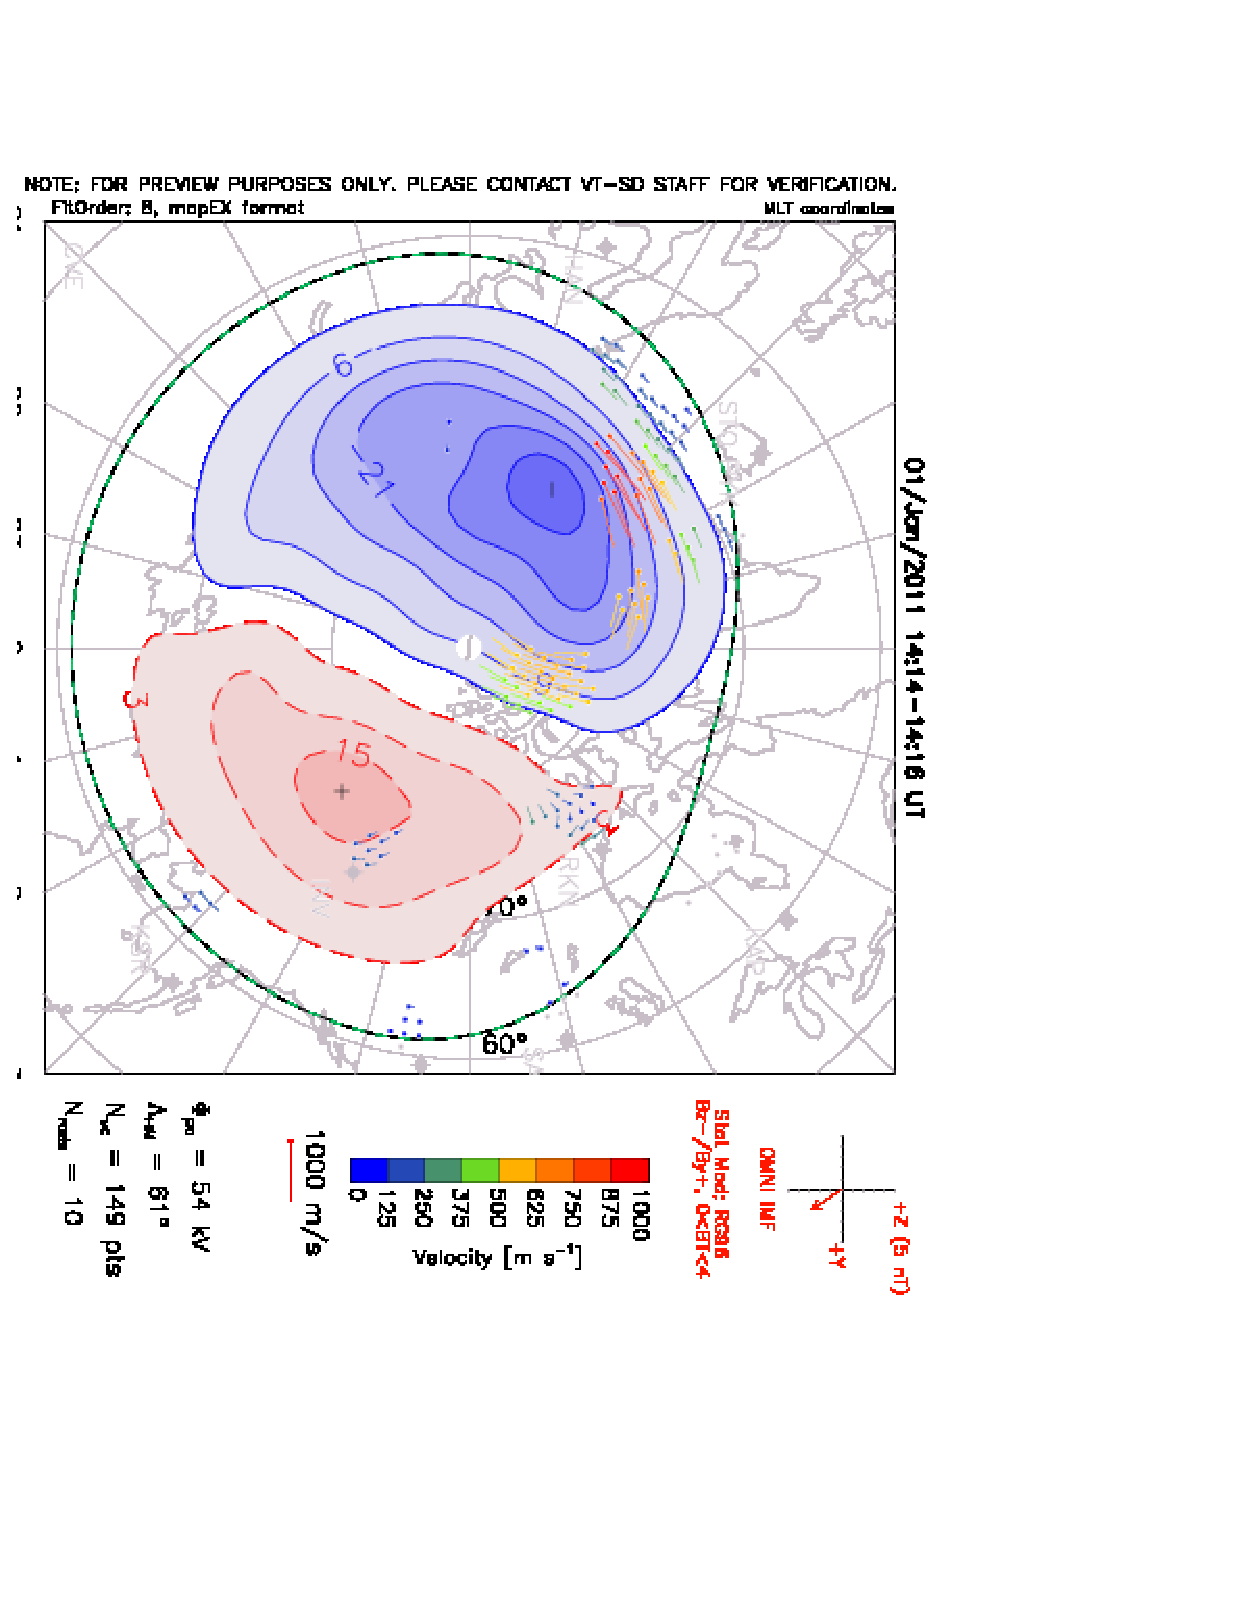
\includegraphics[angle=90,width=\textwidth]{Figures/SD/pot_1415.eps}
\caption{SuperDARN at 14.15}
\label{fig:SD1415}
\end{figure}

\clearpage
\subsection{Current densities (AMPERE)}

In \figref{fig:AMPERE} the current densities from January 1st 2011 between 11.00 to 15.00  calculated from the Irridium satellites are shown. Here the most interesting time is around 14.00 as this is the time with the highest densities. 


\begin{figure}[ht!]

\begin{minipage}{0.33\textwidth}
\includegraphics[width=0.8\textwidth]{Figures/Ampere/1293879600at1100north.pdf}
\caption{11.00}
\end{minipage}
\begin{minipage}{0.33\textwidth}
\includegraphics[width=0.8\textwidth]{Figures/Ampere/1293883200at1200north.pdf}
\caption{12.00}
\end{minipage}
\begin{minipage}{0.33\textwidth}
\includegraphics[width=0.8\textwidth]{Figures/Ampere/1293886800north.pdf}
\caption{13.00}
\end{minipage}

\begin{minipage}{0.33\textwidth}
\includegraphics[width=0.8\textwidth]{Figures/Ampere/1293890400at1400north.pdf}
\caption{14.00}
\end{minipage}
\begin{minipage}{0.33\textwidth}
\includegraphics[width= 0.8\textwidth]{Figures/Ampere/1293891360at1416north.pdf}
\caption{14.16}
\end{minipage}
\begin{minipage}{0.33\textwidth}
\includegraphics[width=0.8\textwidth]{Figures/Ampere/1293894000north.pdf}
\caption{15.00}
\end{minipage}

\caption{Current densities from 11.00 to 16.00 on January 1st 2011, scale from -1.5 $\frac{uA}{m^2}$ to 1.5 $\frac{uA}{m^2}$ , one figure for each hour and an extra for 14.16}
\label{fig:AMPERE}
\end{figure}

At 14.00 the current is up above Svalbard which is the most interesting place to study due to the all-sky camera. And down a bit further south. On the Canadian side there is down furthest north and out further south. At 12.00 there also is a higher density of outward current above Svalbard. 


\subsection{Aurora}

When looking at the Keograms during the day then there is most activity between 11.00 and 15.00. So these will be the ones considered. Starting in the time period between 11.00 and 12.00 then it's possible to see some activity???????

In the keograms the 


\begin{figure}

%%\begin{minipage}{0.49\textwidth}
%%\includegraphics[width = \textwidth]{Figures/Allsky/5577/nya4_20110101_0000_2400_5577_cal.png}
%%\end{minipage}
%%\begin{minipage}{0.49\textwidth}
%%\includegraphics[width=\textwidth]{Figures/Allsky/6300/nya4_20110101_0000_2400_6300_cal.png}
%%\end{minipage}


\begin{minipage}{0.24\textwidth}
\includegraphics[width=\textwidth]{Figures/Allsky/5577/nya4_20110101_1100_1200_5577_cal.png}
\end{minipage}
\begin{minipage}{0.24\textwidth}
\includegraphics[width=\textwidth]{Figures/Allsky/5577/nya4_20110101_1200_1300_5577_cal.png}
\end{minipage}
\begin{minipage}{0.24\textwidth}
\includegraphics[width=\textwidth]{Figures/Allsky/6300/nya4_20110101_1100_1200_6300_cal.png}
\end{minipage}
\begin{minipage}{0.24\textwidth}
\includegraphics[width=\textwidth]{Figures/Allsky/6300/nya4_20110101_1200_1300_6300_cal.png}
\end{minipage}

\begin{minipage}{0.24\textwidth}
\includegraphics[width=\textwidth]{Figures/Allsky/5577/nya4_20110101_1300_1400_5577_cal.png}
\end{minipage}
\begin{minipage}{0.24\textwidth}
\includegraphics[width=\textwidth]{Figures/Allsky/5577/nya4_20110101_1400_1500_5577_cal.png}
\end{minipage}
\begin{minipage}{0.24\textwidth}
\includegraphics[width=\textwidth]{Figures/Allsky/6300/nya4_20110101_1300_1400_6300_cal.png}
\end{minipage}
\begin{minipage}{0.24\textwidth}
\includegraphics[width=\textwidth]{Figures/Allsky/6300/nya4_20110101_1400_1500_6300_cal.png}
\end{minipage}


\caption{Keograms for the time period between 11.00 and 15.00. The four on the left side is in the 5577\AA and the four on the right is in 6300 \AA}
\end{figure}

